\chapter{用户调研}


\section{技术探针}
为了方便进行用户调研,我们选用了云中医app作为技术探针。云中医是复旦大学计算机学院张文强老师和上海中医药大学合作开发的一款面诊应用,主要为诊所环境使用考虑,虽然没有考虑到用户日常长期使用的情况,但是它实现了面诊,舌诊和问诊的基本功能,符合技术探针的要求。云中医是一个手机上的健康诊断应用程序,旨在提供一个方便的平台的自我诊断和健康管理。该应用以中医“四诊”理论为指导,用户需要依次对自己的面部和舌头进行拍照,回答一些与自己健康状况相关的问题,最终会收到一份完整的健康报告和一些健康建议。
云中医app的主要界面如 所示。

\begin{figure}
    \centering
    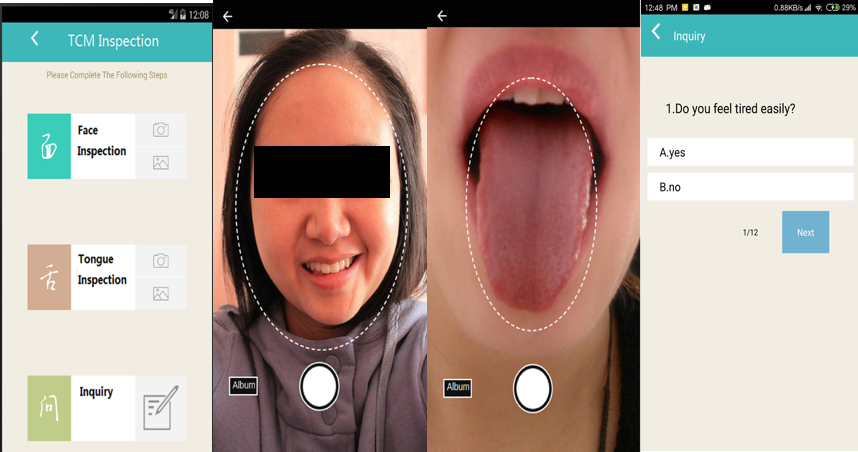
\includegraphics{images/main.png}
    \caption{云中医}
    \label{fig:main}
\end{figure}

\section{调研过程}
 
我们采用定性研究的方法进行半结构化的深度访谈,通过社交媒体发布海报,最终招募到了10位感兴趣的志愿者。招募到合适的用户之后,我们会进行一次采访,主要是为了了解用户信息,介绍技术探针。接下来两周时间,在第一星期,我们不做任何干预。而第二星期,要求用户每天至少使用一次。在用户使用结束后,我们会进行一次结束后的回访,了解用户在使用中遇到的问题和他们的想法;我们希望通过此次调研了解到使用面诊应用的用户群体有哪些?用户期望通过面诊应用来获取哪方面的信息?以及在方便用户日常使用上,有哪些待解决的技术难点?

\begin{table}
  \caption{参与者}
  \centering
  \label{tab:Participants}
  \begin{tabular}{cccl}
编号 &	性别 &	年龄 &	职业 \\
P1 &	男 &	20多 &	博士生 \\
P2 &	男 &	20多 &	研究生 \\
P3 &	男 &	20多 &	研究生 \\
P4 &	女 &	50多 &	医院护理工 \\
P5 &	男 &	40多 &	办公室职员 \\
P6 &	女 &	40多 &	小学老师 \\
P7 &	女 &	50多 &	办公室职员 \\
P8 &	女 &	19岁 &	本科生 \\
P9 &	男 &	20多 &	办公室职员 \\
P10 &	女 &	40多 &	办公室职员 \\
  \end{tabular}
\end{table}

\section{调研发现}
\subsection{潜在的使用场景}
通过调研,我们发现面诊类应用在日常使用环境下,用户反馈有两种潜在的使用场景:

1.了解身体状态
对于那些已经有健康问题的用户或者日常有养生活动的用户对云中医更加感兴趣,并且知道如何在日常生活中使用它。

2.医患沟通的工具
正如其他健康跟踪类技术的发现类似,参与者希望云中一能够提供医生和患者沟通的渠道,这样医生可以更好地获取病人的日常健康信息。

\subsection{自适应性}
日常环境和诊所环境不同,日常环境下需要用户长期使用。但是,大部分的参与者在使用云中医一到两次后就不再使用了,其中一个重要的原因就是云中医缺乏自适应性的能力。自适应性主要体现在两个方面:

1.自适应用户信息
从调研反馈来看,我们发现因为云中医在问诊的时候,一直问用户同样的问题,而实际情况是短期内来说,大部分问题的答案是不会发生改变的,这样缺乏用户信息的自适应性会让用户使用起来觉得很繁琐。

2.自适应环境信息
系统给出的养生建议也是固定的,并没有考虑到用户当前的工作状态和环境因素。中医认为,于环境变化和谐相处对于保持健康很重要,特别是在季节变化的时候。
\subsection{实用性}
1.中医术语
 因为中医中包含大量的中医术语,在日常环境下,用户在使用的时候,周围是没有专业的医生可以询问的,因此通俗易懂的解释中医术语是非常重要的。
 
2.养生建议合理性
不同职业的用户,日常的空余时间是不同的。空余时间是否充裕,是影响用户实践养生建议的关键。因此系统给出的养生建议,特别是需要花费较长时间的按摩熬粥之类大的养生活动,需要合理考虑用户的日常空余时间。
\subsection{敏感性}
1.文化敏感性
舌诊的时候,需要用户伸出舌头进行拍照。在中国文化中,伸出舌头可以表示厌恶或者无礼,因此在很多情况下,在公众场合伸出自己的舌头被认为是不合适的。如P1认为,伸出舌头拍舌头的照片是很不雅的。P3表示自己在和别人拍照的时候都会感到紧张,使用云中医时都是私下使用。因此,文化敏感性限制了该类应用的使用范围。

2.技术敏感性
由于模型需要对面部舌部图片进行颜色特征的提取,使其对外部因素如光照和手机摄像头的质量会更加敏感。P8还特别反映了自己用的时vivo手机,拍照会受到相机自带美颜算法的影响。因此,将面诊应用日常环境下,需要考虑个人设备的因素。

3.社交敏感性
虽然有几位参与者希望分享它们的健康结果给其他人作为相互学习的机会,但是他们同时也担心因为涉及到面部照片和个人健康信息,可能会导致隐私泄露的问题。有趣的是,我们发现和其他社交分享类应用不同的是,对于家人来说,他们更加愿意分享给陌生人,因为分享给家人的话可能会引起家人不必要的担心。
